\panel{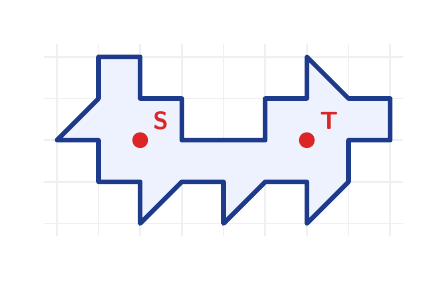
\begin{tikzpicture}[x=1bp, y=1bp]\path[use as bounding box] (0,0) rectangle (141.00,81.00);\clip (0,0) rectangle (141.00,81.00);
\path[draw={rgb,255:red,238;green,240;blue,243}, line width=0.52bp, line cap=round, line join=round] (10.50,6.00) -- (10.50,75.00);
\path[draw={rgb,255:red,238;green,240;blue,243}, line width=0.52bp, line cap=round, line join=round] (25.50,6.00) -- (25.50,75.00);
\path[draw={rgb,255:red,238;green,240;blue,243}, line width=0.52bp, line cap=round, line join=round] (40.50,6.00) -- (40.50,75.00);
\path[draw={rgb,255:red,238;green,240;blue,243}, line width=0.52bp, line cap=round, line join=round] (55.50,6.00) -- (55.50,75.00);
\path[draw={rgb,255:red,238;green,240;blue,243}, line width=0.52bp, line cap=round, line join=round] (70.50,6.00) -- (70.50,75.00);
\path[draw={rgb,255:red,238;green,240;blue,243}, line width=0.52bp, line cap=round, line join=round] (85.50,6.00) -- (85.50,75.00);
\path[draw={rgb,255:red,238;green,240;blue,243}, line width=0.52bp, line cap=round, line join=round] (100.50,6.00) -- (100.50,75.00);
\path[draw={rgb,255:red,238;green,240;blue,243}, line width=0.52bp, line cap=round, line join=round] (115.50,6.00) -- (115.50,75.00);
\path[draw={rgb,255:red,238;green,240;blue,243}, line width=0.52bp, line cap=round, line join=round] (130.50,6.00) -- (130.50,75.00);
\path[draw={rgb,255:red,238;green,240;blue,243}, line width=0.52bp, line cap=round, line join=round] (6.00,10.50) -- (135.00,10.50);
\path[draw={rgb,255:red,238;green,240;blue,243}, line width=0.52bp, line cap=round, line join=round] (6.00,25.50) -- (135.00,25.50);
\path[draw={rgb,255:red,238;green,240;blue,243}, line width=0.52bp, line cap=round, line join=round] (6.00,40.50) -- (135.00,40.50);
\path[draw={rgb,255:red,238;green,240;blue,243}, line width=0.52bp, line cap=round, line join=round] (6.00,55.50) -- (135.00,55.50);
\path[draw={rgb,255:red,238;green,240;blue,243}, line width=0.52bp, line cap=round, line join=round] (6.00,70.50) -- (135.00,70.50);
\path[draw={rgb,255:red,30;green,58;blue,138}, line width=1.65bp, fill={rgb,255:red,238;green,242;blue,255}, line join=round] (10.50,40.50) -- (25.50,40.50) -- (25.50,25.50) -- (40.50,25.50) -- (40.50,10.50) -- (55.50,25.50) -- (70.50,25.50) -- (70.50,10.50) -- (85.50,25.50) -- (100.50,25.50) -- (100.50,10.50) -- (115.50,25.50) -- (115.50,40.50) -- (130.50,40.50) -- (130.50,55.50) -- (115.50,55.50) -- (100.50,70.50) -- (100.50,55.50) -- (85.50,55.50) -- (85.50,40.50) -- (55.50,40.50) -- (55.50,55.50) -- (40.50,55.50) -- (40.50,70.50) -- (25.50,70.50) -- (25.50,55.50) -- cycle;
\path[fill={rgb,255:red,220;green,38;blue,38}] (40.50,40.50) circle[radius=2.85bp];
\node[anchor=base west, text={rgb,255:red,220;green,38;blue,38}, font=\fontsize{9.0}{10.8}\selectfont\sffamily\bfseries, inner sep=0pt] at (45.00,44.25) {S};
\path[fill={rgb,255:red,220;green,38;blue,38}] (100.50,40.50) circle[radius=2.85bp];
\node[anchor=base west, text={rgb,255:red,220;green,38;blue,38}, font=\fontsize{9.0}{10.8}\selectfont\sffamily\bfseries, inner sep=0pt] at (105.00,44.25) {T};
\end{tikzpicture}}{(a) Tokarsky, 1995: 26 walls}\hspace{22.5bp}\panel{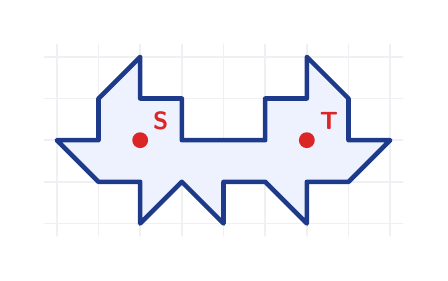
\begin{tikzpicture}[x=1bp, y=1bp]\path[use as bounding box] (0,0) rectangle (141.00,81.00);\clip (0,0) rectangle (141.00,81.00);
\path[draw={rgb,255:red,238;green,240;blue,243}, line width=0.52bp, line cap=round, line join=round] (10.50,6.00) -- (10.50,75.00);
\path[draw={rgb,255:red,238;green,240;blue,243}, line width=0.52bp, line cap=round, line join=round] (25.50,6.00) -- (25.50,75.00);
\path[draw={rgb,255:red,238;green,240;blue,243}, line width=0.52bp, line cap=round, line join=round] (40.50,6.00) -- (40.50,75.00);
\path[draw={rgb,255:red,238;green,240;blue,243}, line width=0.52bp, line cap=round, line join=round] (55.50,6.00) -- (55.50,75.00);
\path[draw={rgb,255:red,238;green,240;blue,243}, line width=0.52bp, line cap=round, line join=round] (70.50,6.00) -- (70.50,75.00);
\path[draw={rgb,255:red,238;green,240;blue,243}, line width=0.52bp, line cap=round, line join=round] (85.50,6.00) -- (85.50,75.00);
\path[draw={rgb,255:red,238;green,240;blue,243}, line width=0.52bp, line cap=round, line join=round] (100.50,6.00) -- (100.50,75.00);
\path[draw={rgb,255:red,238;green,240;blue,243}, line width=0.52bp, line cap=round, line join=round] (115.50,6.00) -- (115.50,75.00);
\path[draw={rgb,255:red,238;green,240;blue,243}, line width=0.52bp, line cap=round, line join=round] (130.50,6.00) -- (130.50,75.00);
\path[draw={rgb,255:red,238;green,240;blue,243}, line width=0.52bp, line cap=round, line join=round] (6.00,10.50) -- (135.00,10.50);
\path[draw={rgb,255:red,238;green,240;blue,243}, line width=0.52bp, line cap=round, line join=round] (6.00,25.50) -- (135.00,25.50);
\path[draw={rgb,255:red,238;green,240;blue,243}, line width=0.52bp, line cap=round, line join=round] (6.00,40.50) -- (135.00,40.50);
\path[draw={rgb,255:red,238;green,240;blue,243}, line width=0.52bp, line cap=round, line join=round] (6.00,55.50) -- (135.00,55.50);
\path[draw={rgb,255:red,238;green,240;blue,243}, line width=0.52bp, line cap=round, line join=round] (6.00,70.50) -- (135.00,70.50);
\path[draw={rgb,255:red,30;green,58;blue,138}, line width=1.65bp, fill={rgb,255:red,238;green,242;blue,255}, line join=round] (10.50,40.50) -- (25.50,25.50) -- (40.50,25.50) -- (40.50,10.50) -- (55.50,25.50) -- (70.50,10.50) -- (70.50,25.50) -- (85.50,25.50) -- (100.50,10.50) -- (100.50,25.50) -- (115.50,25.50) -- (130.50,40.50) -- (115.50,40.50) -- (115.50,55.50) -- (100.50,70.50) -- (100.50,55.50) -- (85.50,55.50) -- (85.50,40.50) -- (55.50,40.50) -- (55.50,55.50) -- (40.50,55.50) -- (40.50,70.50) -- (25.50,55.50) -- (25.50,40.50) -- cycle;
\path[fill={rgb,255:red,220;green,38;blue,38}] (40.50,40.50) circle[radius=2.85bp];
\node[anchor=base west, text={rgb,255:red,220;green,38;blue,38}, font=\fontsize{9.0}{10.8}\selectfont\sffamily\bfseries, inner sep=0pt] at (45.00,44.25) {S};
\path[fill={rgb,255:red,220;green,38;blue,38}] (100.50,40.50) circle[radius=2.85bp];
\node[anchor=base west, text={rgb,255:red,220;green,38;blue,38}, font=\fontsize{9.0}{10.8}\selectfont\sffamily\bfseries, inner sep=0pt] at (105.00,44.25) {T};
\end{tikzpicture}}{(b) Castro, 1997: 24 walls}\hspace{22.5bp}\panel{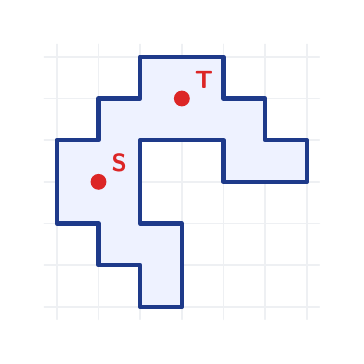
\begin{tikzpicture}[x=1bp, y=1bp]\path[use as bounding box] (0,0) rectangle (111.00,111.00);\clip (0,0) rectangle (111.00,111.00);
\path[draw={rgb,255:red,238;green,240;blue,243}, line width=0.52bp, line cap=round, line join=round] (10.50,6.00) -- (10.50,105.00);
\path[draw={rgb,255:red,238;green,240;blue,243}, line width=0.52bp, line cap=round, line join=round] (25.50,6.00) -- (25.50,105.00);
\path[draw={rgb,255:red,238;green,240;blue,243}, line width=0.52bp, line cap=round, line join=round] (40.50,6.00) -- (40.50,105.00);
\path[draw={rgb,255:red,238;green,240;blue,243}, line width=0.52bp, line cap=round, line join=round] (55.50,6.00) -- (55.50,105.00);
\path[draw={rgb,255:red,238;green,240;blue,243}, line width=0.52bp, line cap=round, line join=round] (70.50,6.00) -- (70.50,105.00);
\path[draw={rgb,255:red,238;green,240;blue,243}, line width=0.52bp, line cap=round, line join=round] (85.50,6.00) -- (85.50,105.00);
\path[draw={rgb,255:red,238;green,240;blue,243}, line width=0.52bp, line cap=round, line join=round] (100.50,6.00) -- (100.50,105.00);
\path[draw={rgb,255:red,238;green,240;blue,243}, line width=0.52bp, line cap=round, line join=round] (6.00,10.50) -- (105.00,10.50);
\path[draw={rgb,255:red,238;green,240;blue,243}, line width=0.52bp, line cap=round, line join=round] (6.00,25.50) -- (105.00,25.50);
\path[draw={rgb,255:red,238;green,240;blue,243}, line width=0.52bp, line cap=round, line join=round] (6.00,40.50) -- (105.00,40.50);
\path[draw={rgb,255:red,238;green,240;blue,243}, line width=0.52bp, line cap=round, line join=round] (6.00,55.50) -- (105.00,55.50);
\path[draw={rgb,255:red,238;green,240;blue,243}, line width=0.52bp, line cap=round, line join=round] (6.00,70.50) -- (105.00,70.50);
\path[draw={rgb,255:red,238;green,240;blue,243}, line width=0.52bp, line cap=round, line join=round] (6.00,85.50) -- (105.00,85.50);
\path[draw={rgb,255:red,238;green,240;blue,243}, line width=0.52bp, line cap=round, line join=round] (6.00,100.50) -- (105.00,100.50);
\path[draw={rgb,255:red,30;green,58;blue,138}, line width=1.65bp, fill={rgb,255:red,238;green,242;blue,255}, line join=round] (10.50,40.50) -- (10.50,70.50) -- (25.50,70.50) -- (25.50,85.50) -- (40.50,85.50) -- (40.50,100.50) -- (70.50,100.50) -- (70.50,85.50) -- (85.50,85.50) -- (85.50,70.50) -- (100.50,70.50) -- (100.50,55.50) -- (70.50,55.50) -- (70.50,70.50) -- (40.50,70.50) -- (40.50,40.50) -- (55.50,40.50) -- (55.50,10.50) -- (40.50,10.50) -- (40.50,25.50) -- (25.50,25.50) -- (25.50,40.50) -- cycle;
\path[fill={rgb,255:red,220;green,38;blue,38}] (25.50,55.50) circle[radius=2.85bp];
\node[anchor=base west, text={rgb,255:red,220;green,38;blue,38}, font=\fontsize{9.0}{10.8}\selectfont\sffamily\bfseries, inner sep=0pt] at (30.00,59.25) {S};
\path[fill={rgb,255:red,220;green,38;blue,38}] (55.50,85.50) circle[radius=2.85bp];
\node[anchor=base west, text={rgb,255:red,220;green,38;blue,38}, font=\fontsize{9.0}{10.8}\selectfont\sffamily\bfseries, inner sep=0pt] at (60.00,89.25) {T};
\end{tikzpicture}}{(c) Your room: 22 walls}
